% Options for packages loaded elsewhere
\PassOptionsToPackage{unicode}{hyperref}
\PassOptionsToPackage{hyphens}{url}
%
\documentclass[
]{article}
\usepackage{amsmath,amssymb}
\usepackage{iftex}
\ifPDFTeX
  \usepackage[T1]{fontenc}
  \usepackage[utf8]{inputenc}
  \usepackage{textcomp} % provide euro and other symbols
\else % if luatex or xetex
  \usepackage{unicode-math} % this also loads fontspec
  \defaultfontfeatures{Scale=MatchLowercase}
  \defaultfontfeatures[\rmfamily]{Ligatures=TeX,Scale=1}
\fi
\usepackage{lmodern}
\ifPDFTeX\else
  % xetex/luatex font selection
\fi
% Use upquote if available, for straight quotes in verbatim environments
\IfFileExists{upquote.sty}{\usepackage{upquote}}{}
\IfFileExists{microtype.sty}{% use microtype if available
  \usepackage[]{microtype}
  \UseMicrotypeSet[protrusion]{basicmath} % disable protrusion for tt fonts
}{}
\makeatletter
\@ifundefined{KOMAClassName}{% if non-KOMA class
  \IfFileExists{parskip.sty}{%
    \usepackage{parskip}
  }{% else
    \setlength{\parindent}{0pt}
    \setlength{\parskip}{6pt plus 2pt minus 1pt}}
}{% if KOMA class
  \KOMAoptions{parskip=half}}
\makeatother
\usepackage{xcolor}
\usepackage[margin=1in]{geometry}
\usepackage{longtable,booktabs,array}
\usepackage{calc} % for calculating minipage widths
% Correct order of tables after \paragraph or \subparagraph
\usepackage{etoolbox}
\makeatletter
\patchcmd\longtable{\par}{\if@noskipsec\mbox{}\fi\par}{}{}
\makeatother
% Allow footnotes in longtable head/foot
\IfFileExists{footnotehyper.sty}{\usepackage{footnotehyper}}{\usepackage{footnote}}
\makesavenoteenv{longtable}
\usepackage{graphicx}
\makeatletter
\def\maxwidth{\ifdim\Gin@nat@width>\linewidth\linewidth\else\Gin@nat@width\fi}
\def\maxheight{\ifdim\Gin@nat@height>\textheight\textheight\else\Gin@nat@height\fi}
\makeatother
% Scale images if necessary, so that they will not overflow the page
% margins by default, and it is still possible to overwrite the defaults
% using explicit options in \includegraphics[width, height, ...]{}
\setkeys{Gin}{width=\maxwidth,height=\maxheight,keepaspectratio}
% Set default figure placement to htbp
\makeatletter
\def\fps@figure{htbp}
\makeatother
\setlength{\emergencystretch}{3em} % prevent overfull lines
\providecommand{\tightlist}{%
  \setlength{\itemsep}{0pt}\setlength{\parskip}{0pt}}
\setcounter{secnumdepth}{5}
\newlength{\cslhangindent}
\setlength{\cslhangindent}{1.5em}
\newlength{\csllabelwidth}
\setlength{\csllabelwidth}{3em}
\newlength{\cslentryspacingunit} % times entry-spacing
\setlength{\cslentryspacingunit}{\parskip}
\newenvironment{CSLReferences}[2] % #1 hanging-ident, #2 entry spacing
 {% don't indent paragraphs
  \setlength{\parindent}{0pt}
  % turn on hanging indent if param 1 is 1
  \ifodd #1
  \let\oldpar\par
  \def\par{\hangindent=\cslhangindent\oldpar}
  \fi
  % set entry spacing
  \setlength{\parskip}{#2\cslentryspacingunit}
 }%
 {}
\usepackage{calc}
\newcommand{\CSLBlock}[1]{#1\hfill\break}
\newcommand{\CSLLeftMargin}[1]{\parbox[t]{\csllabelwidth}{#1}}
\newcommand{\CSLRightInline}[1]{\parbox[t]{\linewidth - \csllabelwidth}{#1}\break}
\newcommand{\CSLIndent}[1]{\hspace{\cslhangindent}#1}
\usepackage{booktabs}
\usepackage{longtable}
\usepackage{amsmath}
\usepackage{graphicx}
\usepackage{float}
\usepackage{booktabs}
\usepackage{longtable}
\usepackage{array}
\usepackage{multirow}
\usepackage{wrapfig}
\usepackage{colortbl}
\usepackage{pdflscape}
\usepackage{tabu}
\usepackage{threeparttable}
\usepackage{threeparttablex}
\usepackage[normalem]{ulem}
\usepackage{makecell}
\usepackage{xcolor}
\ifLuaTeX
  \usepackage{selnolig}  % disable illegal ligatures
\fi
\IfFileExists{bookmark.sty}{\usepackage{bookmark}}{\usepackage{hyperref}}
\IfFileExists{xurl.sty}{\usepackage{xurl}}{} % add URL line breaks if available
\urlstyle{same}
\hypersetup{
  pdftitle={Analyzing Baseball Platoon Strategies: Integrating Bat Speed, Swing Length, Spray Angle, Clustering, and Performance Metrics},
  pdfauthor={Wei Chieh Chen},
  hidelinks,
  pdfcreator={LaTeX via pandoc}}

\title{Analyzing Baseball Platoon Strategies: Integrating Bat Speed,
Swing Length, Spray Angle, Clustering, and Performance Metrics}
\author{Wei Chieh Chen}
\date{2025-04-30}

\begin{document}
\maketitle

{
\setcounter{tocdepth}{2}
\tableofcontents
}
\clearpage

\hypertarget{abstract}{%
\section{Abstract}\label{abstract}}

This study analyzes platoon strategies in baseball using 2024 Statcast
data, focusing on bat speed, swing length, attack angle, and batter
performance metrics. We apply multivariate clustering to group batters
by handedness and swing characteristics, followed by a Monte Carlo
simulation to estimate runs scored. Additionally, we calculate
performance metrics (batting average, on-base percentage, slugging
percentage, OPS, and OPS+) for right-handed, left-handed, and switch
hitters against left- and right-handed pitchers, alongside swing
metrics. Results show distinct platoon advantages, with left-handed
batters excelling against right-handed pitchers (OPS+ = 108) and
right-handed batters performing better against left-handed pitchers
(OPS+ = 104). These findings provide actionable insights for optimizing
lineup decisions in professional baseball.

\hypertarget{introduction}{%
\section{Introduction}\label{introduction}}

In baseball, platoon strategies leverage batter-pitcher handedness
matchups to enhance offensive output. Right-handed batters (RHB)
typically perform better against left-handed pitchers (LHP), while
left-handed batters (LHB) excel against right-handed pitchers (RHP)
(Winston et al., 2022). Switch hitters offer flexibility by batting from
either side. Statcast data, with metrics like bat speed, swing length,
and attack angle, enables deeper analysis of these dynamics (Albert,
2024; Petriello, 2024). This study uses 2024 Statcast data to cluster
batters, simulate game outcomes, and measure platoon performance through
batting average (BA), on-base percentage (OBP), slugging percentage
(SLG), OPS, and OPS+, alongside swing characteristics. We aim to provide
insights for optimizing lineup strategies.

\hypertarget{data-and-methods}{%
\section{Data and Methods}\label{data-and-methods}}

\hypertarget{data-source}{%
\subsection{Data Source}\label{data-source}}

We use the
statcast\_pitch\_swing\_data\_20240402\_20241030\_with\_arm\_angle.csv
dataset from the CSAS 2025 Data Challenge, which includes pitch-level
data for the 2024 MLB regular season and playoffs. The dataset contains
701,557 pitches, with key variables such as bat speed (mean = 71.1 mph,
SD = 4.8), swing length (mean = 7.0 ft, SD = 0.6), launch angle (mean =
12.8 degrees, SD = 24.2), launch speed (mean = 87.5 mph, SD = 14.6), and
batter/pitcher handedness (stand, p\_throws). These swing metrics were
introduced by Statcast in 2024 to capture batter mechanics (Petriello,
2024). Additional variables include pitch type (e.g., FF for four-seam
fastballs), event outcomes (events), and contextual variables like
balls, strikes, and runners on base. For league-wide context, we
reference the 2024 Major League Batting Year-by-Year Averages (Baseball
Reference, 2024), which report a league BA of 0.243, OBP of 0.312, and
SLG of 0.399. A detailed data summary, including descriptive statistics
for key variables, is provided in Table A1 in the appendix.

\hypertarget{preprocessing}{%
\subsection{Preprocessing}\label{preprocessing}}

We preprocess the data by:

\begin{itemize}
\tightlist
\item
  Filtering for swing-related pitches (type == ``X'' or specific
  descriptions like ``hit\_into\_play'').
\item
  Calculating spray angle using hit coordinates:
  \(sprayangle = atan2(hc_y - 200, hc_x - 125) \times 180 / \pi\) ,
  adjusted for batter handedness.
\item
  Computing attack angle as the average launch angle of the top 20\% of
  swings by launch speed, fitted with a parabolic model (Marshall,
  2017).
\item
  Calculating plate discipline metrics (Z-Swing\%, O-Swing\%, Swing\%)
  based on swing decisions in and out of the strike zone.
\end{itemize}

\hypertarget{clustering-analysis}{%
\subsection{Clustering Analysis}\label{clustering-analysis}}

We aggregate batter-level summaries by player, pitch type, and pitcher
handedness, calculating mean bat speed, swing length, attack angle,
spray angle, and estimated BA (eBA) and SLG (eSLG). To reduce
dimensionality, we apply Principal Component Analysis (PCA), retaining
the first four principal components, which capture the majority of
variance in the data (Abdi \& Williams, 2010). We then perform k-means
clustering (k=4) separately for right-handed batters (RHB) and
left-handed batters (LHB), resulting in eight distinct clusters.

Labeling of Clusters: The clusters for right-handed batters are labeled
RHB-1, RHB-2, RHB-3, and RHB-4, where the prefix ``RHB'' indicates
right-handed batters, and the numbers 1 to 4 represent the four distinct
groups identified by the k-means algorithm. Similarly, the clusters for
left-handed batters are labeled LHB-1, LHB-2, LHB-3, and LHB-4, with
``LHB'' denoting left-handed batters.

Cluster Characteristics: Each cluster represents a unique batter profile
based on swing metrics, as observed in Table 1 (four-seam fastball
data): - RHB-1: Contact-oriented hitters with moderate bat speed
(70.9--71.2 mph) and shorter swings (6.9--7.0 ft). They have a low
attack angle (6.2--6.5 degrees), indicating a flatter swing suited for
line drives and ground balls. - RHB-2: Aggressive power hitters with
high bat speed (72.4--72.8 mph) and longer swings (7.3 ft). Their higher
attack angle (15.9 degrees) suggests an upward swing path optimized for
fly balls and home runs. - RHB-3: Compact swingers with lower bat speed
(67.0 mph) and the shortest swings (6.4 ft). Their attack angle (7.6
degrees) indicates a focus on contact hitting with minimal loft. -
RHB-4: Balanced hitters with moderate bat speed (69.4--69.5 mph) and
swing length (6.8 ft). They have a moderate attack angle (14.8--15.3
degrees), suitable for a mix of power and contact hitting. - LHB-1:
Compact swingers with lower bat speed (65.2--66.0 mph) and shorter
swings (6.3 ft). Their attack angle (10.2--10.7 degrees) suggests a
balanced approach with moderate loft. - LHB-2: Versatile hitters with
moderate bat speed (69.1--69.9 mph) and swing length (6.7 ft). Their
attack angle varies (10.5--12.2 degrees), showing adaptability to
different pitching matchups. - LHB-3: Power hitters with higher bat
speed (70.2--70.6 mph) and moderate swing length (6.8--6.9 ft). They
have the highest attack angle (18.6--20.1 degrees), ideal for generating
lift and power, especially against RHP. - LHB-4: Aggressive hitters with
the highest bat speed (72.3--73.4 mph) and moderate swing length
(6.8--6.9 ft). Their attack angle (13.7--13.8 degrees) supports a
power-hitting profile with consistent loft.

These clusters help identify distinct batter profiles, which can inform
scouting, player development, and lineup strategies by highlighting
strengths in specific platoon matchups.

\hypertarget{monte-carlo-simulation}{%
\subsection{Monte Carlo Simulation}\label{monte-carlo-simulation}}

We estimate event probabilities (e.g., home run, strikeout, walk,
single) for each cluster based on their mean estimated BA (eBA),
estimated SLG (eSLG), and wOBA, derived from the Statcast data. These
probabilities are calculated using a simplified model where, for
example, the probability of a home run is proportional to wOBA, while
strikeouts and groundouts are based on (1 - eBA), adjusted for realistic
event distributions (e.g., HR probability = 0.2 × wOBA, strikeout
probability = 0.3 × (1 - eBA)). A Monte Carlo simulation is then
conducted to estimate offensive output, running 10,000 simulated games
with a sample lineup.

\begin{itemize}
\tightlist
\item
  Simulation Setup: The sample lineup consists of nine batters
  alternating between RHB and LHB clusters: RHB-1, LHB-2, RHB-4, LHB-1,
  RHB-3, LHB-3, RHB-2, LHB-4, RHB-1. This lineup reflects a balanced
  platoon strategy, mixing different batter profiles to optimize
  performance against a generic opponent (assumed to be a mix of RHP and
  LHP). Each game simulates nine innings, with outcomes (e.g., runs
  scored, outs) determined by sampling from the event probabilities for
  each batter in the lineup. A park factor of 1 is applied, assuming a
  neutral stadium environment (Winston et al., 2022).
\item
  Results and Implications: The simulation estimates an average of
  4.8664 runs per game, which aligns with typical MLB team scoring rates
  (e.g., the 2024 MLB average was approximately 4.5 runs per game per
  team, per Baseball Reference, 2024). This result suggests that the
  alternating platoon lineup leverages handedness advantages
  effectively, as clusters like LHB-3 (power hitters) and RHB-2
  (aggressive swingers) contribute to higher run production against
  opposite-handed pitchers. The simulation provides a baseline for
  expected offensive output, which can be used to evaluate lineup
  configurations and inform in-game decisions, such as substituting
  batters to exploit specific platoon matchups.
\end{itemize}

\hypertarget{platoon-performance-metrics}{%
\subsection{Platoon Performance
Metrics}\label{platoon-performance-metrics}}

We aggregate the data to the plate appearance level by selecting the
last pitch of each PA (using game\_pk, at\_bat\_number, batter). We
classify batters as RHB, LHB, or Switch Hitters based on their stand
values across PAs. Performance metrics are calculated as follows:

\begin{itemize}
\tightlist
\item
  BA: Hits / At-Bats (excluding walks, HBP, sac flies, sac bunts).
\item
  OBP: (Hits + Walks + HBP) / (At-Bats + Walks + HBP + Sac Flies).
\item
  SLG: Total Bases / At-Bats (total bases = 1 for single, 2 for double,
  3 for triple, 4 for home run).
\item
  OPS: OBP + SLG.
\item
  OPS+:
  \(100 \times \left( \frac{\text{OBP}}{\text{lgOBP}} + \frac{\text{SLG}}{\text{lgSLG}} - 1 \right)\),
  where lgOBP = 0.309 and lgSLG = 0.397 (calculated from the dataset).
\end{itemize}

\hypertarget{results}{%
\section{Results}\label{results}}

\hypertarget{clustering-and-simulation-results}{%
\subsection{Clustering and Simulation
Results}\label{clustering-and-simulation-results}}

The PCA scree plot (Figure 2) shows that the first four principal
components explain a significant portion of variance in batter swing
metrics (Abdi \& Williams, 2010). Clustering results (Figure 3) reveal
distinct groups of RHB and LHB, as described in Section 2.3. For
right-handed batters, RHB-2 represents aggressive power hitters with
high bat speed, while RHB-3 includes contact-oriented hitters with
shorter swings. For left-handed batters, LHB-3 features power hitters
with high attack angles, and LHB-1 consists of batters with compact
swings.

Table 1 summarizes the swing characteristics of all 8 clusters against
four-seam fastballs (FF), focusing on bat speed, swing length, and
attack angle. For example, RHB-2 against RHP fastballs has a bat speed
of 72.4 mph, while LHB-3 against RHP fastballs shows a higher attack
angle of 20.1 degrees, suggesting a more upward swing suited for power
hitting. LHB clusters generally exhibit higher attack angles against RHP
(e.g., LHB-3: 20.1 degrees) compared to LHP (e.g., LHB-3: 18.6 degrees),
which may contribute to their platoon advantage against RHP. The full
platoon summary across all pitch types is provided in Table A2 in the
appendix.

The Monte Carlo simulation, detailed in Section 2.4, estimates an
average of 4.8664 runs per game, reflecting realistic offensive output
adjusted for platoon matchups (Winston et al., 2022).

\hypertarget{platoon-performance-analysis}{%
\subsection{Platoon Performance
Analysis}\label{platoon-performance-analysis}}

Tables 2 and 3 (for LHP) and Tables 4 and 5 (for RHP) present the swing
characteristics and performance metrics of RHB, LHB, and Switch Hitters,
respectively. Key findings include:

\begin{itemize}
\tightlist
\item
  vs LHP (Tables 2 and 3): RHB outperform LHB, with an OPS+ of 104
  compared to 89 for LHB. Switch Hitters perform slightly above average
  (OPS+ = 105). RHB also have a higher bat speed (70.6 mph) compared to
  LHB (69.1 mph), though Switch Hitters show a lower attack angle (9.6
  degrees), indicating a flatter swing profile.
\item
  vs RHP (Tables 4 and 5): LHB excel with an OPS+ of 108, while RHB have
  an OPS+ of 95. Switch Hitters are near average (OPS+ = 100). LHB show
  a higher attack angle (12.7 degrees) compared to RHB (11.5 degrees),
  which may contribute to their higher slugging percentage (0.416).
\end{itemize}

\hypertarget{visualization-of-swing-dynamics}{%
\subsection{Visualization of Swing
Dynamics}\label{visualization-of-swing-dynamics}}

Figure 1 illustrates the relationship between bat speed and launch speed
for home runs, showing a positive correlation (Launch Speed = 104.4 +
0.54 × (Bat Speed -- 75)) (Albert, 2024). This linear model assumes a
linear relationship between bat speed and launch speed, suggesting that
higher bat speeds contribute to harder-hit balls, increasing home run
likelihood.

\begin{table}[H]
\centering
\caption{\label{tab:unnamed-chunk-1}Platoon Summary by Cluster for Four-Seam Fastballs (FF)}
\centering
\begin{tabular}[t]{ccccc}
\toprule
Cluster & Pitcher & Bat.Speed..mph. & Swing.Length..ft. & Attack.Angle..deg.\\
\midrule
LHB-1 & LHP & 65.2 & 6.3 & 10.7\\
LHB-1 & RHP & 66.0 & 6.3 & 10.2\\
LHB-2 & LHP & 69.9 & 6.7 & 10.5\\
LHB-2 & RHP & 69.1 & 6.7 & 12.2\\
LHB-3 & LHP & 70.2 & 6.8 & 18.6\\
\addlinespace
LHB-3 & RHP & 70.6 & 6.9 & 20.1\\
LHB-4 & LHP & 72.3 & 6.8 & 13.7\\
LHB-4 & RHP & 73.4 & 6.9 & 13.8\\
RHB-1 & LHP & 71.2 & 6.9 & 6.2\\
RHB-1 & RHP & 70.9 & 7.0 & 6.5\\
\addlinespace
RHB-2 & LHP & 72.8 & 7.3 & 15.9\\
RHB-2 & RHP & 72.4 & 7.3 & 15.9\\
RHB-3 & LHP & 67.0 & 6.4 & 7.6\\
RHB-3 & RHP & 67.0 & 6.4 & 7.6\\
RHB-4 & LHP & 69.5 & 6.8 & 14.8\\
\addlinespace
RHB-4 & RHP & 69.4 & 6.8 & 15.3\\
\bottomrule
\end{tabular}
\end{table}

\begin{table}[H]
\centering
\caption{\label{tab:unnamed-chunk-2}Swing Metrics vs LHP}
\centering
\begin{tabular}[t]{cccc}
\toprule
Batter\_Type & Bat.Speed..mph. & Swing.Length..ft. & Attack.Angle..deg.\\
\midrule
LHB & 69.1 & 7.1 & 12.8\\
RHB & 70.6 & 7.3 & 11.4\\
Switch Hitter & 69.3 & 7.2 & 9.6\\
\bottomrule
\end{tabular}
\end{table}

\begin{table}[H]
\centering
\caption{\label{tab:unnamed-chunk-3}Performance Metrics vs LHP}
\centering
\begin{tabular}[t]{cccccc}
\toprule
Batter\_Type & Batting\_Avg & On\_Base\_Pct & Slugging\_Pct & OPS & OPS\_plus\\
\midrule
LHB & 0.236 & 0.301 & 0.365 & 0.666 & 89\\
RHB & 0.246 & 0.313 & 0.406 & 0.719 & 104\\
Switch Hitter & 0.252 & 0.312 & 0.412 & 0.724 & 105\\
\bottomrule
\end{tabular}
\end{table}

\begin{table}[H]
\centering
\caption{\label{tab:unnamed-chunk-4}Swing Metrics vs RHP}
\centering
\begin{tabular}[t]{cccc}
\toprule
Batter\_Type & Bat.Speed..mph. & Swing.Length..ft. & Attack.Angle..deg.\\
\midrule
LHB & 70.3 & 7.2 & 12.7\\
RHB & 70.1 & 7.3 & 11.5\\
Switch Hitter & 69.0 & 7.1 & 13.6\\
\bottomrule
\end{tabular}
\end{table}

\begin{table}[H]
\centering
\caption{\label{tab:unnamed-chunk-5}Performance Metrics vs RHP}
\centering
\begin{tabular}[t]{cccccc}
\toprule
Batter\_Type & Batting\_Avg & On\_Base\_Pct & Slugging\_Pct & OPS & OPS\_plus\\
\midrule
LHB & 0.244 & 0.318 & 0.416 & 0.734 & 108\\
RHB & 0.239 & 0.301 & 0.386 & 0.687 & 95\\
Switch Hitter & 0.239 & 0.311 & 0.393 & 0.704 & 100\\
\bottomrule
\end{tabular}
\end{table}

\begin{center}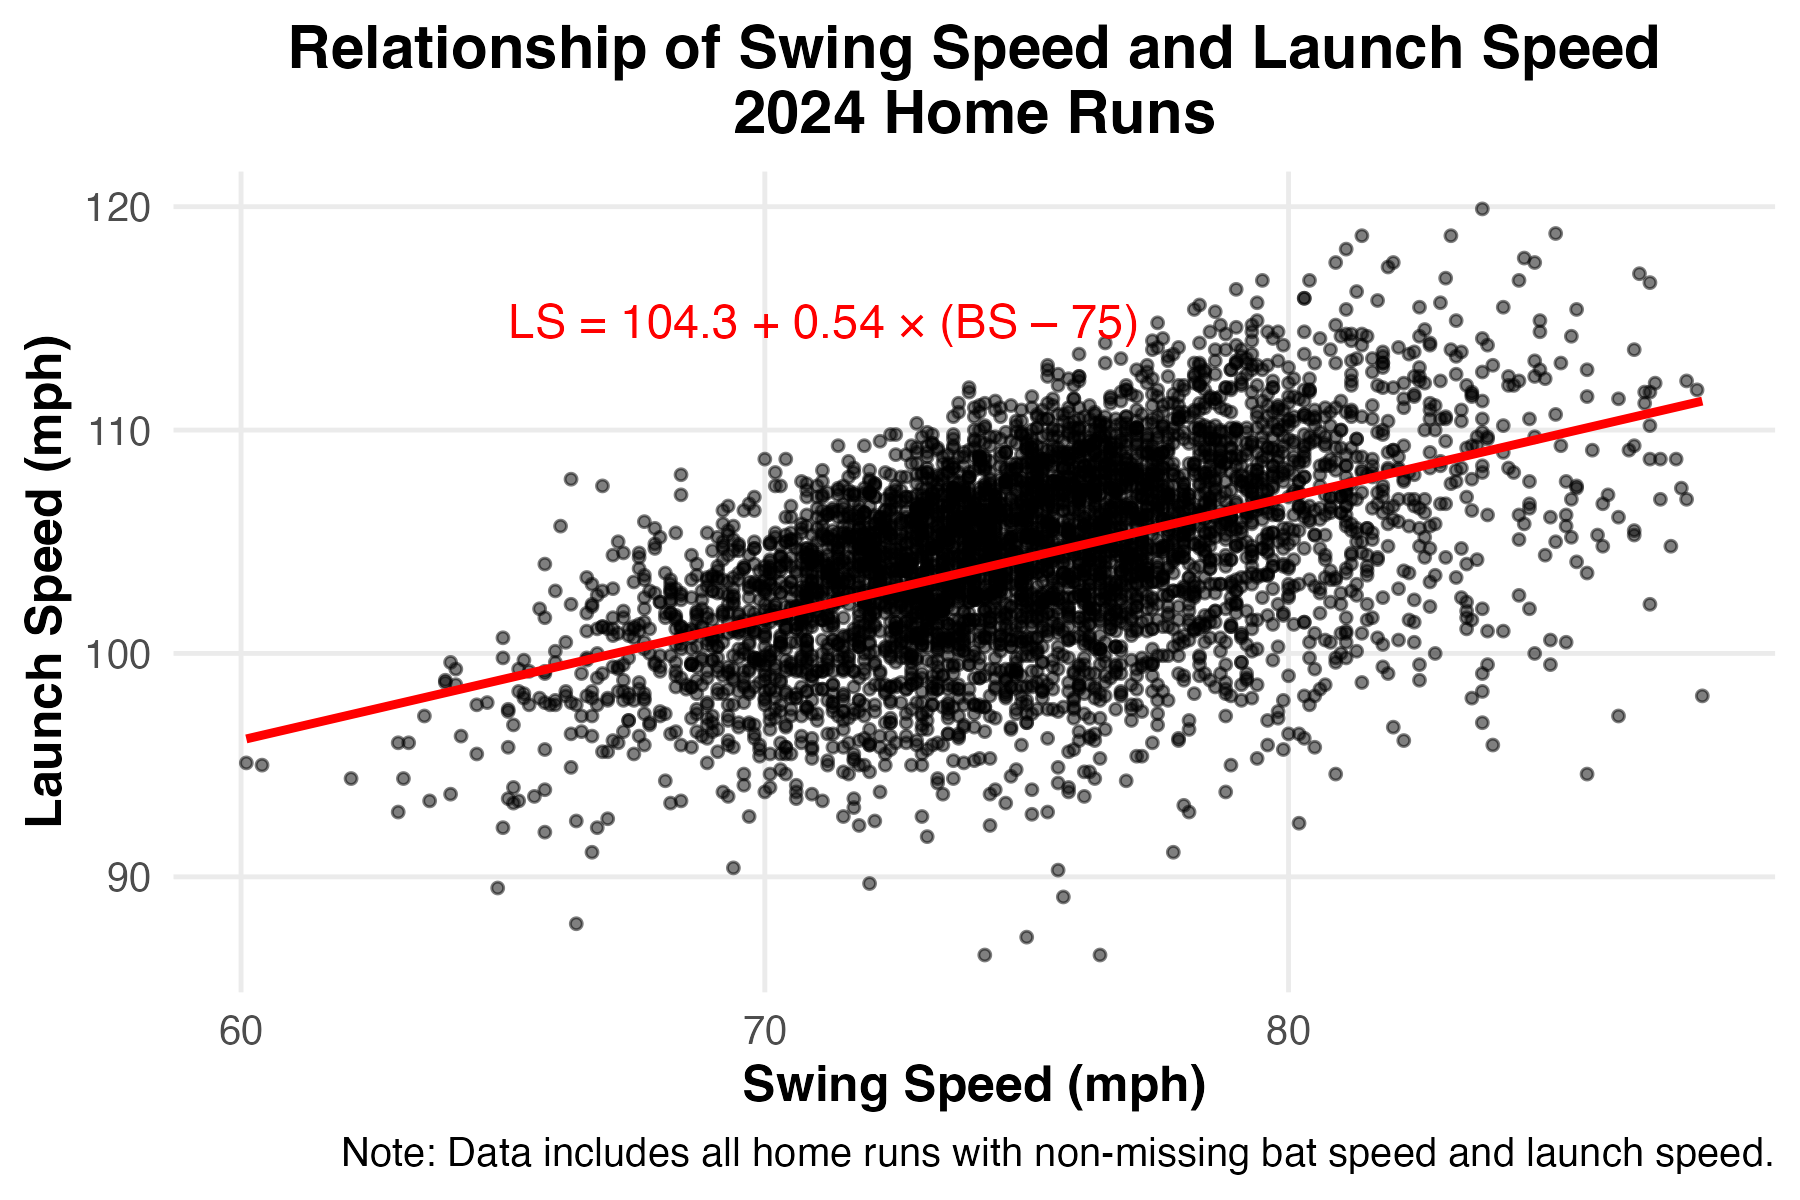
\includegraphics[width=0.4\linewidth]{swing_launch_plot} 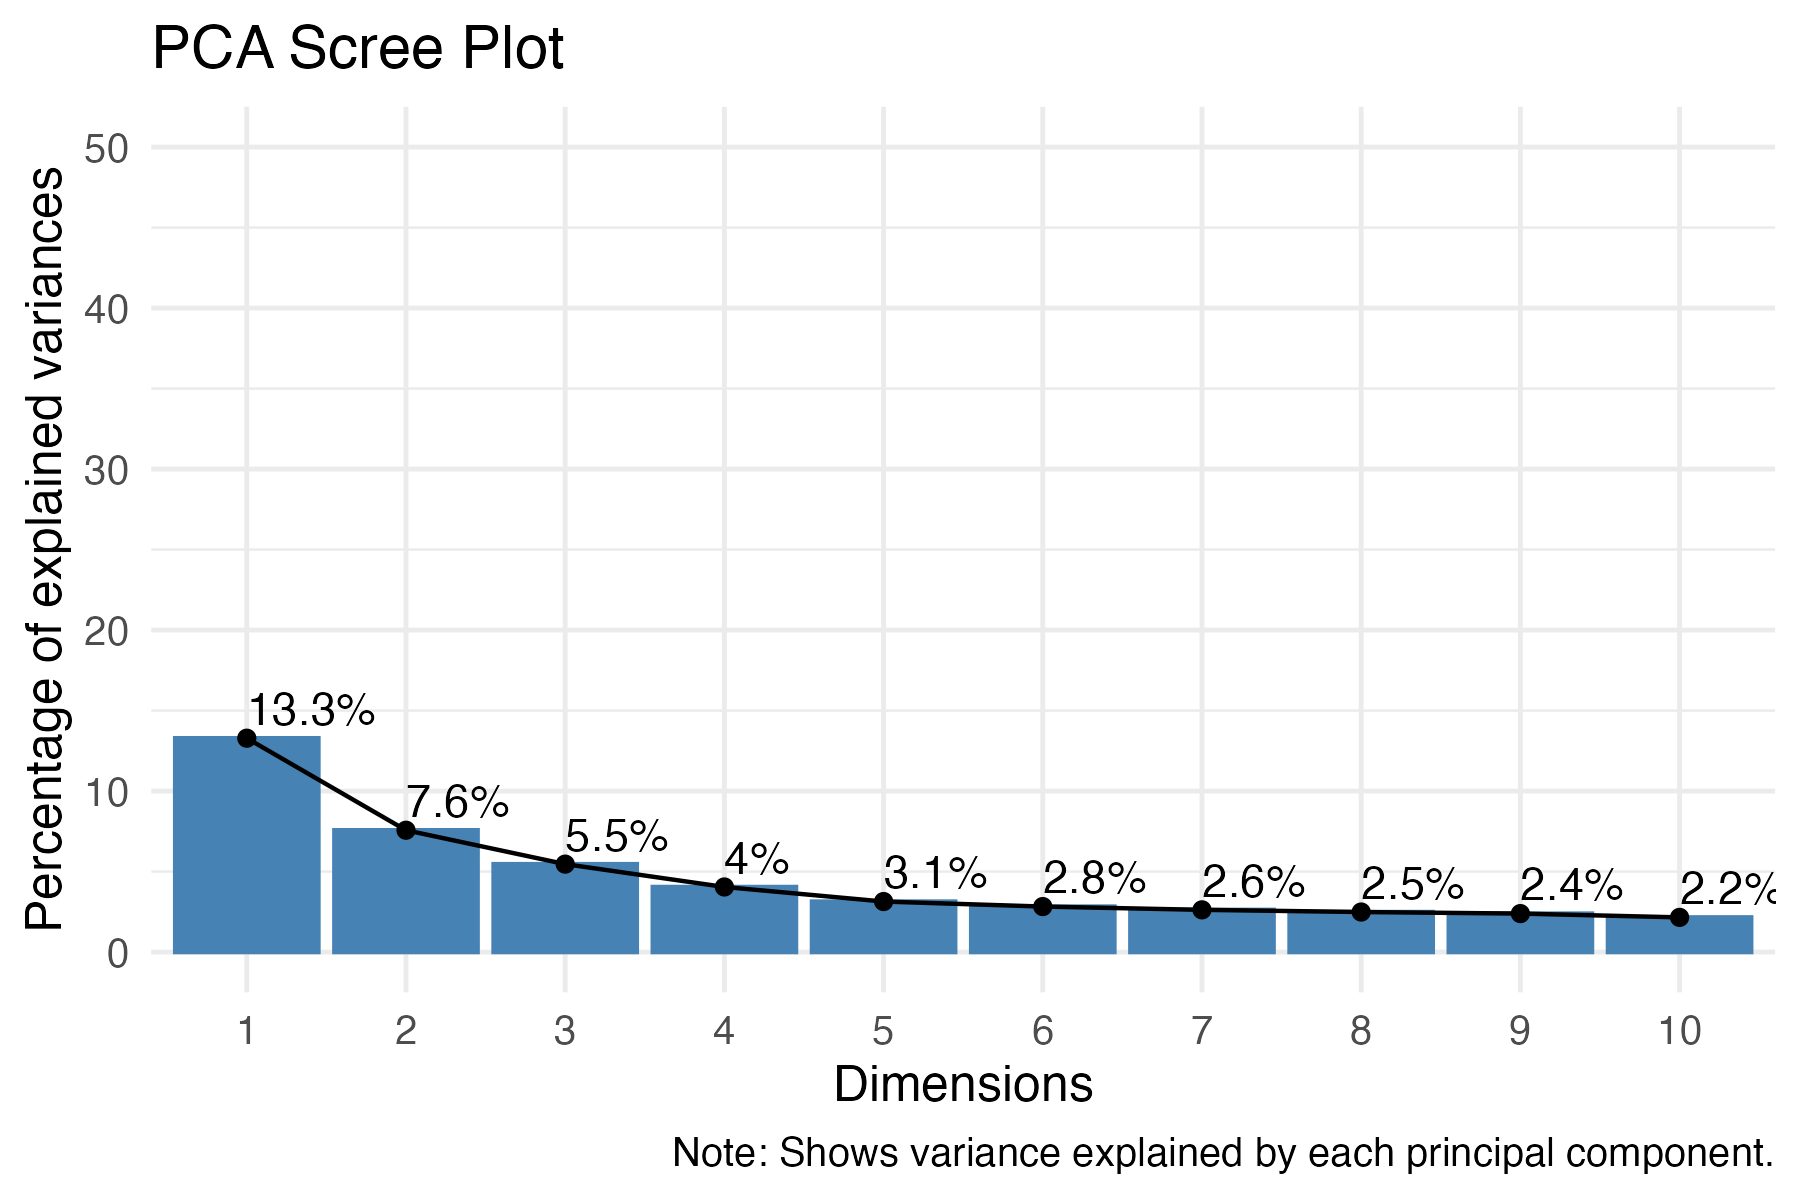
\includegraphics[width=0.4\linewidth]{scree_plot} 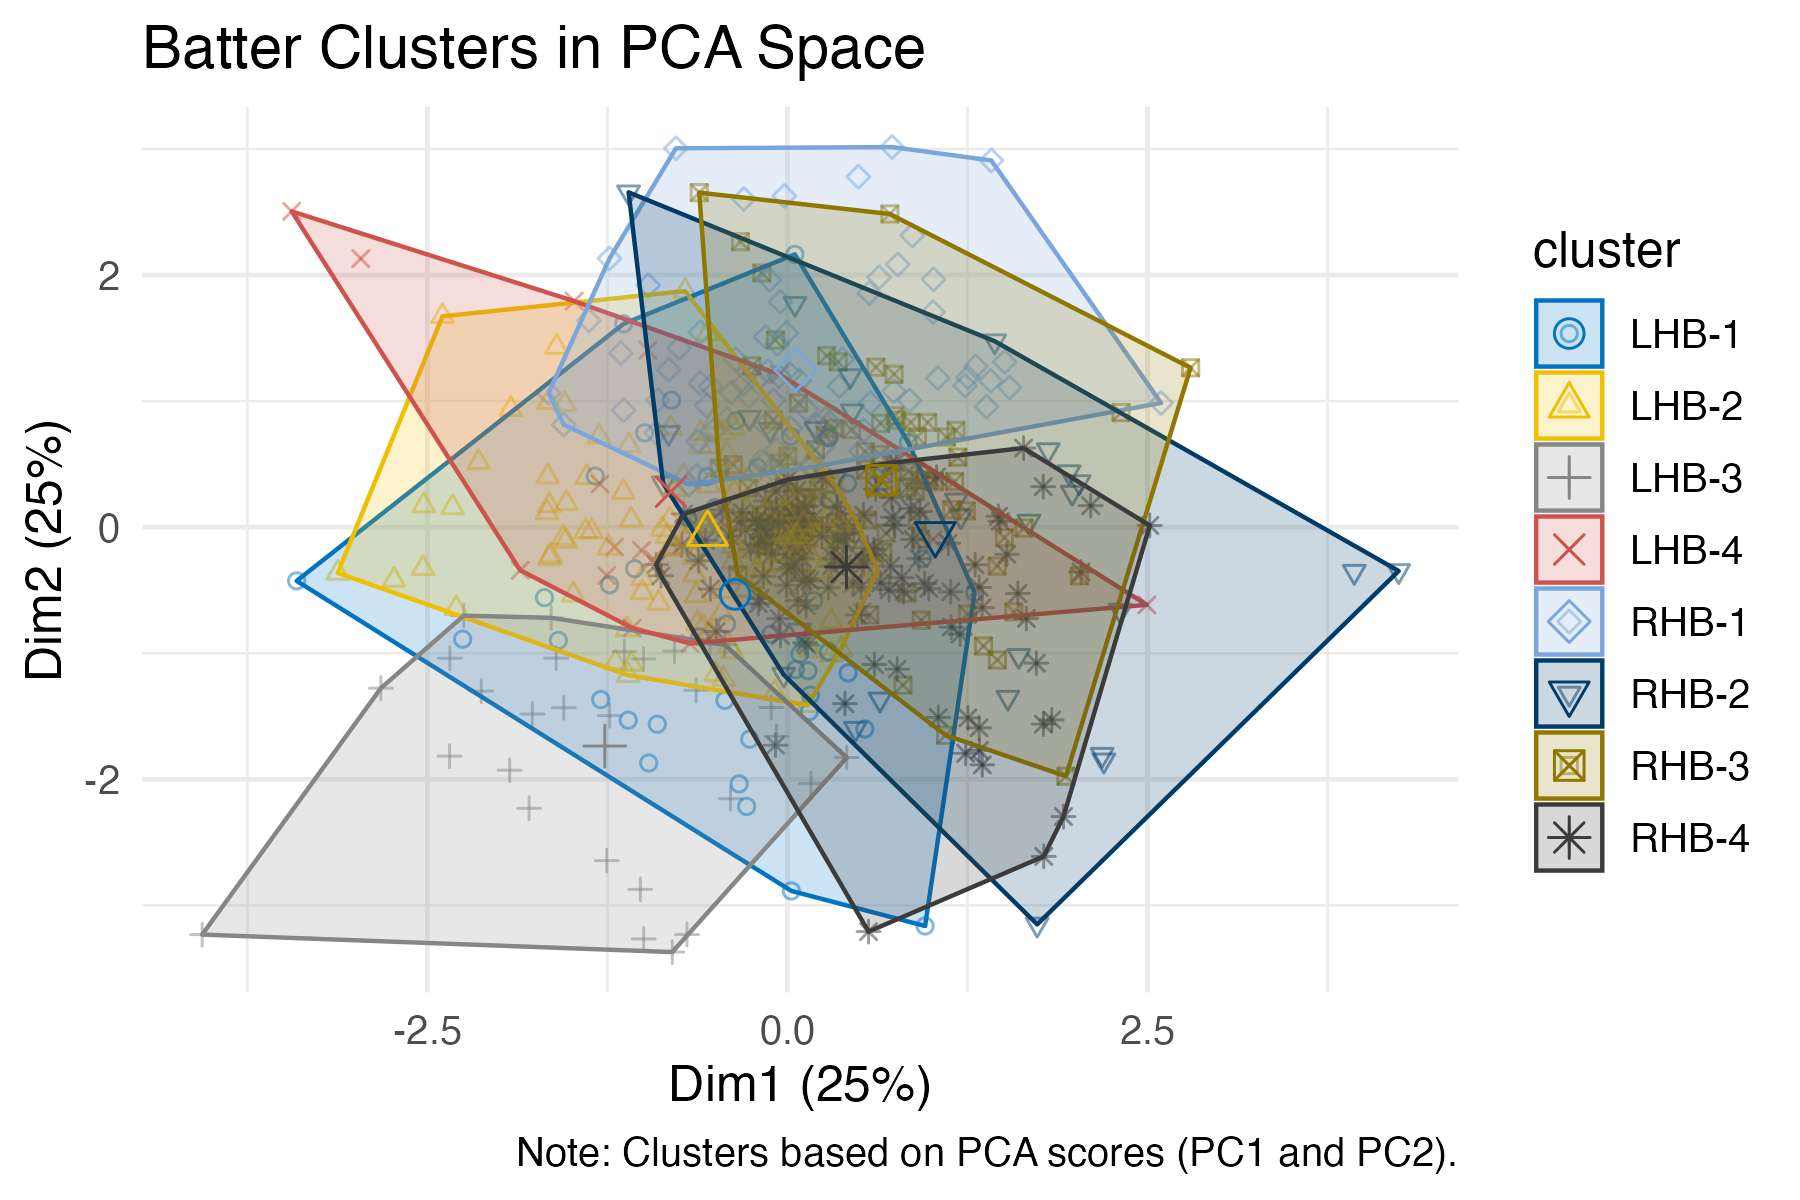
\includegraphics[width=0.4\linewidth]{cluster_plot} \end{center}

\hypertarget{discussion}{%
\section{Discussion}\label{discussion}}

\hypertarget{value-of-the-research}{%
\subsection{Value of the Research}\label{value-of-the-research}}

This study provides a comprehensive framework for understanding platoon
dynamics in baseball, combining advanced swing metrics (bat speed, swing
length, attack angle) with multivariate clustering and traditional
performance metrics (BA, OBP, SLG, OPS, OPS+). The clustering analysis
identifies distinct batter profiles, such as RHB-2 (high bat speed,
aggressive swingers) and LHB-3 (power hitters with high attack angles),
which can inform player development and scouting strategies. The platoon
performance tables (Tables 2 and 3) quantify handedness advantages,
confirming that LHB excel against RHP (OPS+ = 108) and RHB perform
better against LHP (OPS+ = 104). These insights are valuable for
optimizing lineup construction, ensuring managers can maximize offensive
output by exploiting favorable matchups.

\hypertarget{application-to-a-baseball-franchise}{%
\subsection{Application to a Baseball
Franchise}\label{application-to-a-baseball-franchise}}

For a baseball franchise, this research offers practical applications in
several areas:

\begin{itemize}
\tightlist
\item
  Lineup Optimization: Managers can use the platoon performance metrics
  to construct daily lineups that maximize offensive production. For
  example, against an RHP, a team might prioritize LHB with high OPS+
  (e.g., 108) to exploit the platoon advantage, while ensuring Switch
  Hitters (OPS+ = 100) provide balance. The swing metrics in Tables 2
  and 3 (e.g., LHB's attack angle of 12.7 degrees vs RHP) can further
  guide matchup decisions, favoring batters with optimal swing profiles
  for power hitting.
\item
  Player Scouting and Development: The clustering results (e.g., RHB-2
  vs RHB-3) highlight different batter profiles based on bat speed,
  swing length, and attack angle, enabling scouts to target players who
  fit specific team needs (e.g., power hitters for LHP matchups).
  Coaches can also use these metrics to tailor training programs,
  improving players' swing mechanics (Petriello, 2024).
\item
  Game Strategy: The Monte Carlo simulation (4.8664 runs/game) provides
  a baseline for expected offensive output, which can inform in-game
  decisions like pinch-hitting or lineup adjustments. Franchises can
  extend this simulation by incorporating real-time pitcher data to
  refine strategies further.
\end{itemize}

By integrating these findings, a franchise can enhance its competitive
edge, improving both short-term game outcomes and long-term player
development.

\hypertarget{link-to-sports-medicine-injuries-and-load-management}{%
\subsection{Link to Sports Medicine: Injuries and Load
Management}\label{link-to-sports-medicine-injuries-and-load-management}}

Platoon strategies can also be linked to sports medicine, particularly
in the areas of player injuries and load management. By strategically
rotating players based on handedness matchups, teams can manage player
workload, especially during demanding schedules such as consecutive road
games over multiple days. For example:

\begin{itemize}
\tightlist
\item
  Injury Prevention: Clusters like RHB-2 and LHB-4, characterized by
  high bat speed and aggressive swings, may exert greater physical
  stress on players due to the intensity of their swings. Overuse,
  particularly during long road trips, could increase the risk of
  injuries such as muscle strains or fatigue-related issues. Platoon
  strategies that alternate these aggressive hitters with
  contact-oriented players (e.g., RHB-1, LHB-1) could reduce physical
  strain, lowering injury risk.
\item
  Load Management: Consecutive road games place significant physical and
  mental demands on players, including travel fatigue and limited
  recovery time. Platoon strategies can help distribute playing time
  more evenly across the roster, ensuring key players are rested during
  grueling schedules. For instance, a team might rest LHB-3 (power
  hitters) against a tough LHP matchup, preserving their energy for a
  more favorable RHP matchup later in the road trip, thus optimizing
  performance while managing fatigue.
\end{itemize}

This connection highlights the potential of platoon strategies to
contribute to player health and longevity, an area of growing interest
in sports medicine and team management.

\hypertarget{limitations}{%
\subsection{Limitations}\label{limitations}}

Despite its strengths, this study has several limitations. First, the
Monte Carlo simulation simplifies game dynamics by assuming fixed event
probabilities and a static park factor of 1, ignoring variables like
pitcher fatigue, defensive alignments, and situational context (Winston
et al., 2022). Second, the Statcast data may have missing values for bat
speed and swing length, potentially biasing the clustering results.
Third, the inclusion of playoff games slightly lowers overall offensive
metrics (e.g., league BA = 0.242 vs.~0.243 for regular season, as
reported by Baseball Reference, 2024), reflecting stronger pitching in
the postseason, which may not generalize to regular-season strategies.
Fourth, the linear regression model in Figure 1 assumes independence of
observations, but home run data may exhibit dependencies (e.g., multiple
home runs by the same batter or in the same game), which could affect
the model's validity. Finally, the analysis focuses on batter
performance and does not account for pitcher-specific metrics, such as
arm angle variations, which could further refine platoon matchups
(Adler, 2024).

\hypertarget{future-work}{%
\subsection{Future Work}\label{future-work}}

Addressing the limitations of this study opens several avenues for
future research:

\begin{itemize}
\tightlist
\item
  Incorporate Pitcher Metrics: Including pitcher-specific metrics, such
  as arm angle variations, could enhance the accuracy of platoon
  matchups and simulation outcomes (Adler, 2024).
\item
  Model Situational Factors: Future simulations could account for
  dynamic factors like pitcher fatigue, defensive alignments, and game
  situations (e.g., runners on base, inning) to better reflect
  real-world scenarios.
\item
  Integrate Injury Data: To explore the link with sports medicine,
  future work could incorporate injury data to analyze how platoon
  strategies impact player health. For example, tracking injury rates
  for aggressive clusters (e.g., RHB-2, LHB-4) during consecutive road
  games could reveal whether strategic rotation reduces injury risk and
  improves load management. This could involve analyzing medical
  records, game logs, and player workload metrics to quantify the
  relationship between platoon usage, physical stress, and injury
  incidence.
\item
  Regular-Season Focus: Excluding playoff data or adjusting for
  postseason effects could improve the generalizability of findings to
  regular-season strategies.
\end{itemize}

By integrating these elements, future research can provide a more
holistic understanding of platoon strategies, balancing performance
optimization with player health and well-being.

\hypertarget{conclusion}{%
\section{Conclusion}\label{conclusion}}

This study demonstrates the power of Statcast data in analyzing platoon
strategies. By combining swing metrics (bat speed, swing length, attack
angle), clustering, and performance analysis, we provide a framework for
lineup optimization. Future work could incorporate pitcher-specific
metrics, such as arm angle variations (Adler, 2024), to enhance
simulation accuracy.

\hypertarget{ethics}{%
\section{Ethics}\label{ethics}}

This study, part of the CSAS 2025 Data Challenge, follows ethical
principles in data science and sports analytics, ensuring responsible
use of Statcast data and its implications for players and teams.

\begin{itemize}
\item
  \textbf{Data Privacy:} The Statcast dataset
  (\texttt{statcast\_pitch\_swing\_data\_20240402\_20241030\_with\_arm\_angle.csv})
  lacks PII beyond player names. We focused on aggregated statistics
  (e.g., RHB, LHB clusters) to avoid identifying individuals, minimizing
  risks of stigmatization based on swing or platoon performance.
\item
  \textbf{Fairness:} We used objective methods (PCA, k-means, Monte
  Carlo simulation) to cluster batters and assess performance, ensuring
  unbiased analysis. Including regular season and playoff data reduces
  bias across game contexts.
\item
  \textbf{Transparency:} Methods (preprocessing, clustering, simulation)
  are documented in the paper and code (\texttt{platoon\_code.R}),
  meeting Data Challenge reproducibility requirements. Future work with
  additional data will maintain transparency.
\item
  \textbf{Responsible Use:} Findings (e.g., LHB vs RHP: OPS+ = 108; RHB
  vs LHP: OPS+ = 104) aim to optimize lineups, but over-reliance on
  platoon matchups may hinder player development. Teams should balance
  analytics with holistic management to support player growth.
\item
  \textbf{Future Work with Injury Data:} Proposed injury data
  integration raises ethical concerns:

  \begin{itemize}
  \tightlist
  \item
    \textbf{Confidentiality:} Anonymize injury data to protect player
    privacy.
  \item
    \textbf{Consent:} Ensure players consent to using medical data,
    understanding its purpose.
  \item
    \textbf{Stigma:} Avoid labeling players (e.g., RHB-2, LHB-4) as
    ``injury-prone'' by reporting aggregate results.
  \item
    \textbf{Welfare:} Use data to reduce injury risk (e.g., rotating
    aggressive hitters during road games), aligning with sports medicine
    goals.
  \end{itemize}
\item
  \textbf{Compliance:} We adhered to CSAS 2025 Data Challenge
  guidelines, using the provided dataset without modification and
  ensuring reproducibility via documented code.
\end{itemize}

This study responsibly contributes to sports analytics, prioritizing
player well-being alongside performance insights.

\hypertarget{references}{%
\section{References}\label{references}}

\hypertarget{refs}{}
\begin{CSLReferences}{1}{0}
\leavevmode\vadjust pre{\hypertarget{ref-abdi2010principal}{}}%
Abdi, H., \& Williams, L. J. (2010). Principal component analysis.
\emph{Wiley Interdisciplinary Reviews: Computational Statistics},
\emph{2}(4), 433--459. \url{https://doi.org/10.1002/wics.101}

\leavevmode\vadjust pre{\hypertarget{ref-adler2024rainbow}{}}%
Adler, D. (2024). \emph{The rainbow of arm angles in the playoffs}.
\url{https://www.mlb.com/news/the-range-of-pitcher-arm-angles-in-the-2024-mlb-postseason}

\leavevmode\vadjust pre{\hypertarget{ref-albert2024bat}{}}%
Albert, J. (2024). \emph{Bat speed and swing length}.
\url{https://baseballwithr.wordpress.com/2024/05/17/bat-speed-and-swing-length/}

\leavevmode\vadjust pre{\hypertarget{ref-baseballreference2024}{}}%
Baseball Reference. (2024). \emph{2024 MLB standard batting}.
\url{https://www.baseball-reference.com/leagues/majors/bat.shtml}

\leavevmode\vadjust pre{\hypertarget{ref-marshall2017reverse}{}}%
Marshall, D. (2017). \emph{Reverse engineering swing mechanics from
statcast data}.
\url{https://community.fangraphs.com/reverse-engineering-swing-mechanics-from-statcast-data/}

\leavevmode\vadjust pre{\hypertarget{ref-petriello2024statcast}{}}%
Petriello, M. (2024). \emph{Everything to know about statcast's new
bat-tracking data}.
\url{https://www.mlb.com/news/what-you-need-to-know-about-statcast-bat-tracking}

\leavevmode\vadjust pre{\hypertarget{ref-winston2022mathletics}{}}%
Winston, W. L., Nestler, S. T., \& Pelechrinis, K. (2022).
\emph{Mathletics: How gamblers, managers, and fans use mathematics in
sports} (2nd ed.). Princeton University Press.

\end{CSLReferences}

\clearpage

\hypertarget{appendix}{%
\section{Appendix}\label{appendix}}

\hypertarget{data-summary}{%
\subsection{Data Summary}\label{data-summary}}

The dataset contains 701,557 pitches from the 2024 MLB season, including
regular season and playoffs. Table A1 provides descriptive statistics
for key variables used in the analysis, generated using the summarytools
package. Numerical variables like bat speed (mean = 71.1 mph, SD = 4.8)
and swing length (mean = 7.0 ft, SD = 0.6) show the distribution of
swing characteristics, while launch angle and launch speed indicate
batted ball outcomes. Categorical variables like stand (55.3\% R, 44.7\%
L) and p\_throws (70.2\% R, 29.8\% L) reflect the platoon split, and
pitch type highlights the prevalence of four-seam fastballs (FF:
31.8\%).

\hypertarget{data-frame-summary}{%
\subsubsection{Data Frame Summary}\label{data-frame-summary}}

\hypertarget{selected_data}{%
\paragraph{selected\_data}\label{selected_data}}

\textbf{Dimensions:} 701557 x 7\\
\textbf{Duplicates:} 400547

\begin{longtable}[]{@{}
  >{\raggedright\arraybackslash}p{(\columnwidth - 12\tabcolsep) * \real{0.0420}}
  >{\raggedright\arraybackslash}p{(\columnwidth - 12\tabcolsep) * \real{0.1345}}
  >{\raggedright\arraybackslash}p{(\columnwidth - 12\tabcolsep) * \real{0.2269}}
  >{\raggedright\arraybackslash}p{(\columnwidth - 12\tabcolsep) * \real{0.1933}}
  >{\raggedright\arraybackslash}p{(\columnwidth - 12\tabcolsep) * \real{0.1849}}
  >{\raggedright\arraybackslash}p{(\columnwidth - 12\tabcolsep) * \real{0.0924}}
  >{\raggedright\arraybackslash}p{(\columnwidth - 12\tabcolsep) * \real{0.0840}}@{}}
\toprule\noalign{}
\begin{minipage}[b]{\linewidth}\raggedright
No
\end{minipage} & \begin{minipage}[b]{\linewidth}\raggedright
Variable
\end{minipage} & \begin{minipage}[b]{\linewidth}\raggedright
Stats / Values
\end{minipage} & \begin{minipage}[b]{\linewidth}\raggedright
Freqs (\% of Valid)
\end{minipage} & \begin{minipage}[b]{\linewidth}\raggedright
Graph
\end{minipage} & \begin{minipage}[b]{\linewidth}\raggedright
Valid
\end{minipage} & \begin{minipage}[b]{\linewidth}\raggedright
Missing
\end{minipage} \\
\midrule\noalign{}
\endhead
\bottomrule\noalign{}
\endlastfoot
1 & \begin{minipage}[t]{\linewidth}\raggedright
bat\_speed\\
{[}numeric{]}\strut
\end{minipage} & \begin{minipage}[t]{\linewidth}\raggedright
Mean (sd) : 69.5 (8.9)\\
min \textless{} med \textless{} max:\\
0.9 \textless{} 70.9 \textless{} 88\\
IQR (CV) : 7.3 (0.1)\strut
\end{minipage} & 869 distinct values & 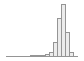
\includegraphics{tmp/ds0050.png}
& \begin{minipage}[t]{\linewidth}\raggedright
322556\\
(46.0\%)\strut
\end{minipage} & \begin{minipage}[t]{\linewidth}\raggedright
379001\\
(54.0\%)\strut
\end{minipage} \\
2 & \begin{minipage}[t]{\linewidth}\raggedright
swing\_length\\
{[}numeric{]}\strut
\end{minipage} & \begin{minipage}[t]{\linewidth}\raggedright
Mean (sd) : 7.2 (1)\\
min \textless{} med \textless{} max:\\
0.3 \textless{} 7.3 \textless{} 12\\
IQR (CV) : 1.3 (0.1)\strut
\end{minipage} & 106 distinct values & 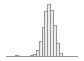
\includegraphics{tmp/ds0051.png}
& \begin{minipage}[t]{\linewidth}\raggedright
322556\\
(46.0\%)\strut
\end{minipage} & \begin{minipage}[t]{\linewidth}\raggedright
379001\\
(54.0\%)\strut
\end{minipage} \\
3 & \begin{minipage}[t]{\linewidth}\raggedright
launch\_angle\\
{[}numeric{]}\strut
\end{minipage} & \begin{minipage}[t]{\linewidth}\raggedright
Mean (sd) : 17.5 (32.9)\\
min \textless{} med \textless{} max:\\
-90 \textless{} 20 \textless{} 90\\
IQR (CV) : 46 (1.9)\strut
\end{minipage} & 181 distinct values & 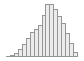
\includegraphics{tmp/ds0052.png}
& \begin{minipage}[t]{\linewidth}\raggedright
235339\\
(33.5\%)\strut
\end{minipage} & \begin{minipage}[t]{\linewidth}\raggedright
466218\\
(66.5\%)\strut
\end{minipage} \\
4 & \begin{minipage}[t]{\linewidth}\raggedright
launch\_speed\\
{[}numeric{]}\strut
\end{minipage} & \begin{minipage}[t]{\linewidth}\raggedright
Mean (sd) : 82.5 (15.2)\\
min \textless{} med \textless{} max:\\
3 \textless{} 82.1 \textless{} 121.5\\
IQR (CV) : 21.3 (0.2)\strut
\end{minipage} & 1116 distinct values & 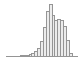
\includegraphics{tmp/ds0053.png}
& \begin{minipage}[t]{\linewidth}\raggedright
235030\\
(33.5\%)\strut
\end{minipage} & \begin{minipage}[t]{\linewidth}\raggedright
466527\\
(66.5\%)\strut
\end{minipage} \\
5 & \begin{minipage}[t]{\linewidth}\raggedright
stand\\
{[}character{]}\strut
\end{minipage} & \begin{minipage}[t]{\linewidth}\raggedright
1. L\\
2. R\strut
\end{minipage} & \begin{minipage}[t]{\linewidth}\raggedright
301866 (43.0\%)\\
399691 (57.0\%)\strut
\end{minipage} & 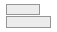
\includegraphics{tmp/ds0054.png} &
\begin{minipage}[t]{\linewidth}\raggedright
701557\\
(100.0\%)\strut
\end{minipage} & \begin{minipage}[t]{\linewidth}\raggedright
0\\
(0.0\%)\strut
\end{minipage} \\
6 & \begin{minipage}[t]{\linewidth}\raggedright
p\_throws\\
{[}character{]}\strut
\end{minipage} & \begin{minipage}[t]{\linewidth}\raggedright
1. L\\
2. R\strut
\end{minipage} & \begin{minipage}[t]{\linewidth}\raggedright
188354 (26.8\%)\\
513203 (73.2\%)\strut
\end{minipage} & 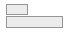
\includegraphics{tmp/ds0055.png} &
\begin{minipage}[t]{\linewidth}\raggedright
701557\\
(100.0\%)\strut
\end{minipage} & \begin{minipage}[t]{\linewidth}\raggedright
0\\
(0.0\%)\strut
\end{minipage} \\
7 & \begin{minipage}[t]{\linewidth}\raggedright
pitch\_type\\
{[}character{]}\strut
\end{minipage} & \begin{minipage}[t]{\linewidth}\raggedright
1. FF\\
2. SI\\
3. SL\\
4. CH\\
5. FC\\
6. CU\\
7. ST\\
8. FS\\
9. KC\\
10. SV\\
{[} 8 others {]}\strut
\end{minipage} & \begin{minipage}[t]{\linewidth}\raggedright
223099 (31.8\%)\\
111928 (16.0\%)\\
111052 (15.8\%)\\
71466 (10.2\%)\\
57172 ( 8.1\%)\\
46005 ( 6.6\%)\\
42650 ( 6.1\%)\\
21043 ( 3.0\%)\\
11692 ( 1.7\%)\\
2645 ( 0.4\%)\\
2805 ( 0.4\%)\strut
\end{minipage} & 
\includegraphics{tmp/ds0056.png} &
\begin{minipage}[t]{\linewidth}\raggedright
701557\\
(100.0\%)\strut
\end{minipage} & \begin{minipage}[t]{\linewidth}\raggedright
0\\
(0.0\%)\strut
\end{minipage} \\
\end{longtable}

\hypertarget{full-platoon-summary-by-cluster-pitch-type-and-pitcher-handedness}{%
\subsection{Full Platoon Summary by Cluster, Pitch Type, and Pitcher
Handedness}\label{full-platoon-summary-by-cluster-pitch-type-and-pitcher-handedness}}

\begin{table}[H]
\centering
\caption{\label{tab:unnamed-chunk-6}Full Platoon Summary by Cluster, Pitch Type, and Pitcher Handedness}
\centering
\begin{tabular}[t]{cccccc}
\toprule
Cluster & Pitch\_Type & Pitcher & Bat.Speed..mph. & Swing.Length..ft. & Attack.Angle..deg.\\
\midrule
LHB-1 & FF & LHP & 65.2 & 6.3 & 10.7\\
LHB-1 & FF & RHP & 66.0 & 6.3 & 10.2\\
LHB-1 & SL & LHP & 63.7 & 7.1 & 10.8\\
LHB-1 & SL & RHP & 66.7 & 7.2 & 10.2\\
LHB-2 & FF & LHP & 69.9 & 6.7 & 10.5\\
\addlinespace
LHB-2 & FF & RHP & 69.1 & 6.7 & 12.2\\
LHB-2 & SL & LHP & 67.5 & 7.2 & 10.5\\
LHB-2 & SL & RHP & 69.9 & 7.3 & 12.2\\
LHB-3 & FF & LHP & 70.2 & 6.8 & 18.6\\
LHB-3 & FF & RHP & 70.6 & 6.9 & 20.1\\
\addlinespace
LHB-3 & SL & LHP & 67.8 & 7.2 & 18.6\\
LHB-3 & SL & RHP & 70.9 & 7.4 & 20.1\\
LHB-4 & FF & LHP & 72.3 & 6.8 & 13.7\\
LHB-4 & FF & RHP & 73.4 & 6.9 & 13.8\\
LHB-4 & SL & LHP & 70.5 & 7.2 & 13.7\\
\addlinespace
LHB-4 & SL & RHP & 73.5 & 7.4 & 13.8\\
RHB-1 & FF & LHP & 71.2 & 6.9 & 6.2\\
RHB-1 & FF & RHP & 70.9 & 7.0 & 6.5\\
RHB-1 & SL & LHP & 69.2 & 7.2 & 6.2\\
RHB-1 & SL & RHP & 71.3 & 7.3 & 6.5\\
\addlinespace
RHB-2 & FF & LHP & 72.8 & 7.3 & 15.9\\
RHB-2 & FF & RHP & 72.4 & 7.3 & 15.9\\
RHB-2 & SL & LHP & 70.7 & 7.6 & 15.9\\
RHB-2 & SL & RHP & 72.5 & 7.7 & 15.9\\
RHB-3 & FF & LHP & 67.0 & 6.4 & 7.6\\
\addlinespace
RHB-3 & FF & RHP & 67.0 & 6.4 & 7.6\\
RHB-3 & SL & LHP & 65.3 & 7.0 & 7.6\\
RHB-3 & SL & RHP & 67.1 & 7.1 & 7.6\\
RHB-4 & FF & LHP & 69.5 & 6.8 & 14.8\\
RHB-4 & FF & RHP & 69.4 & 6.8 & 15.3\\
\addlinespace
RHB-4 & SL & LHP & 67.6 & 7.2 & 14.8\\
RHB-4 & SL & RHP & 69.5 & 7.3 & 15.3\\
\bottomrule
\end{tabular}
\end{table}

\hypertarget{additional-visualizations}{%
\subsection{Additional Visualizations}\label{additional-visualizations}}

\begin{center}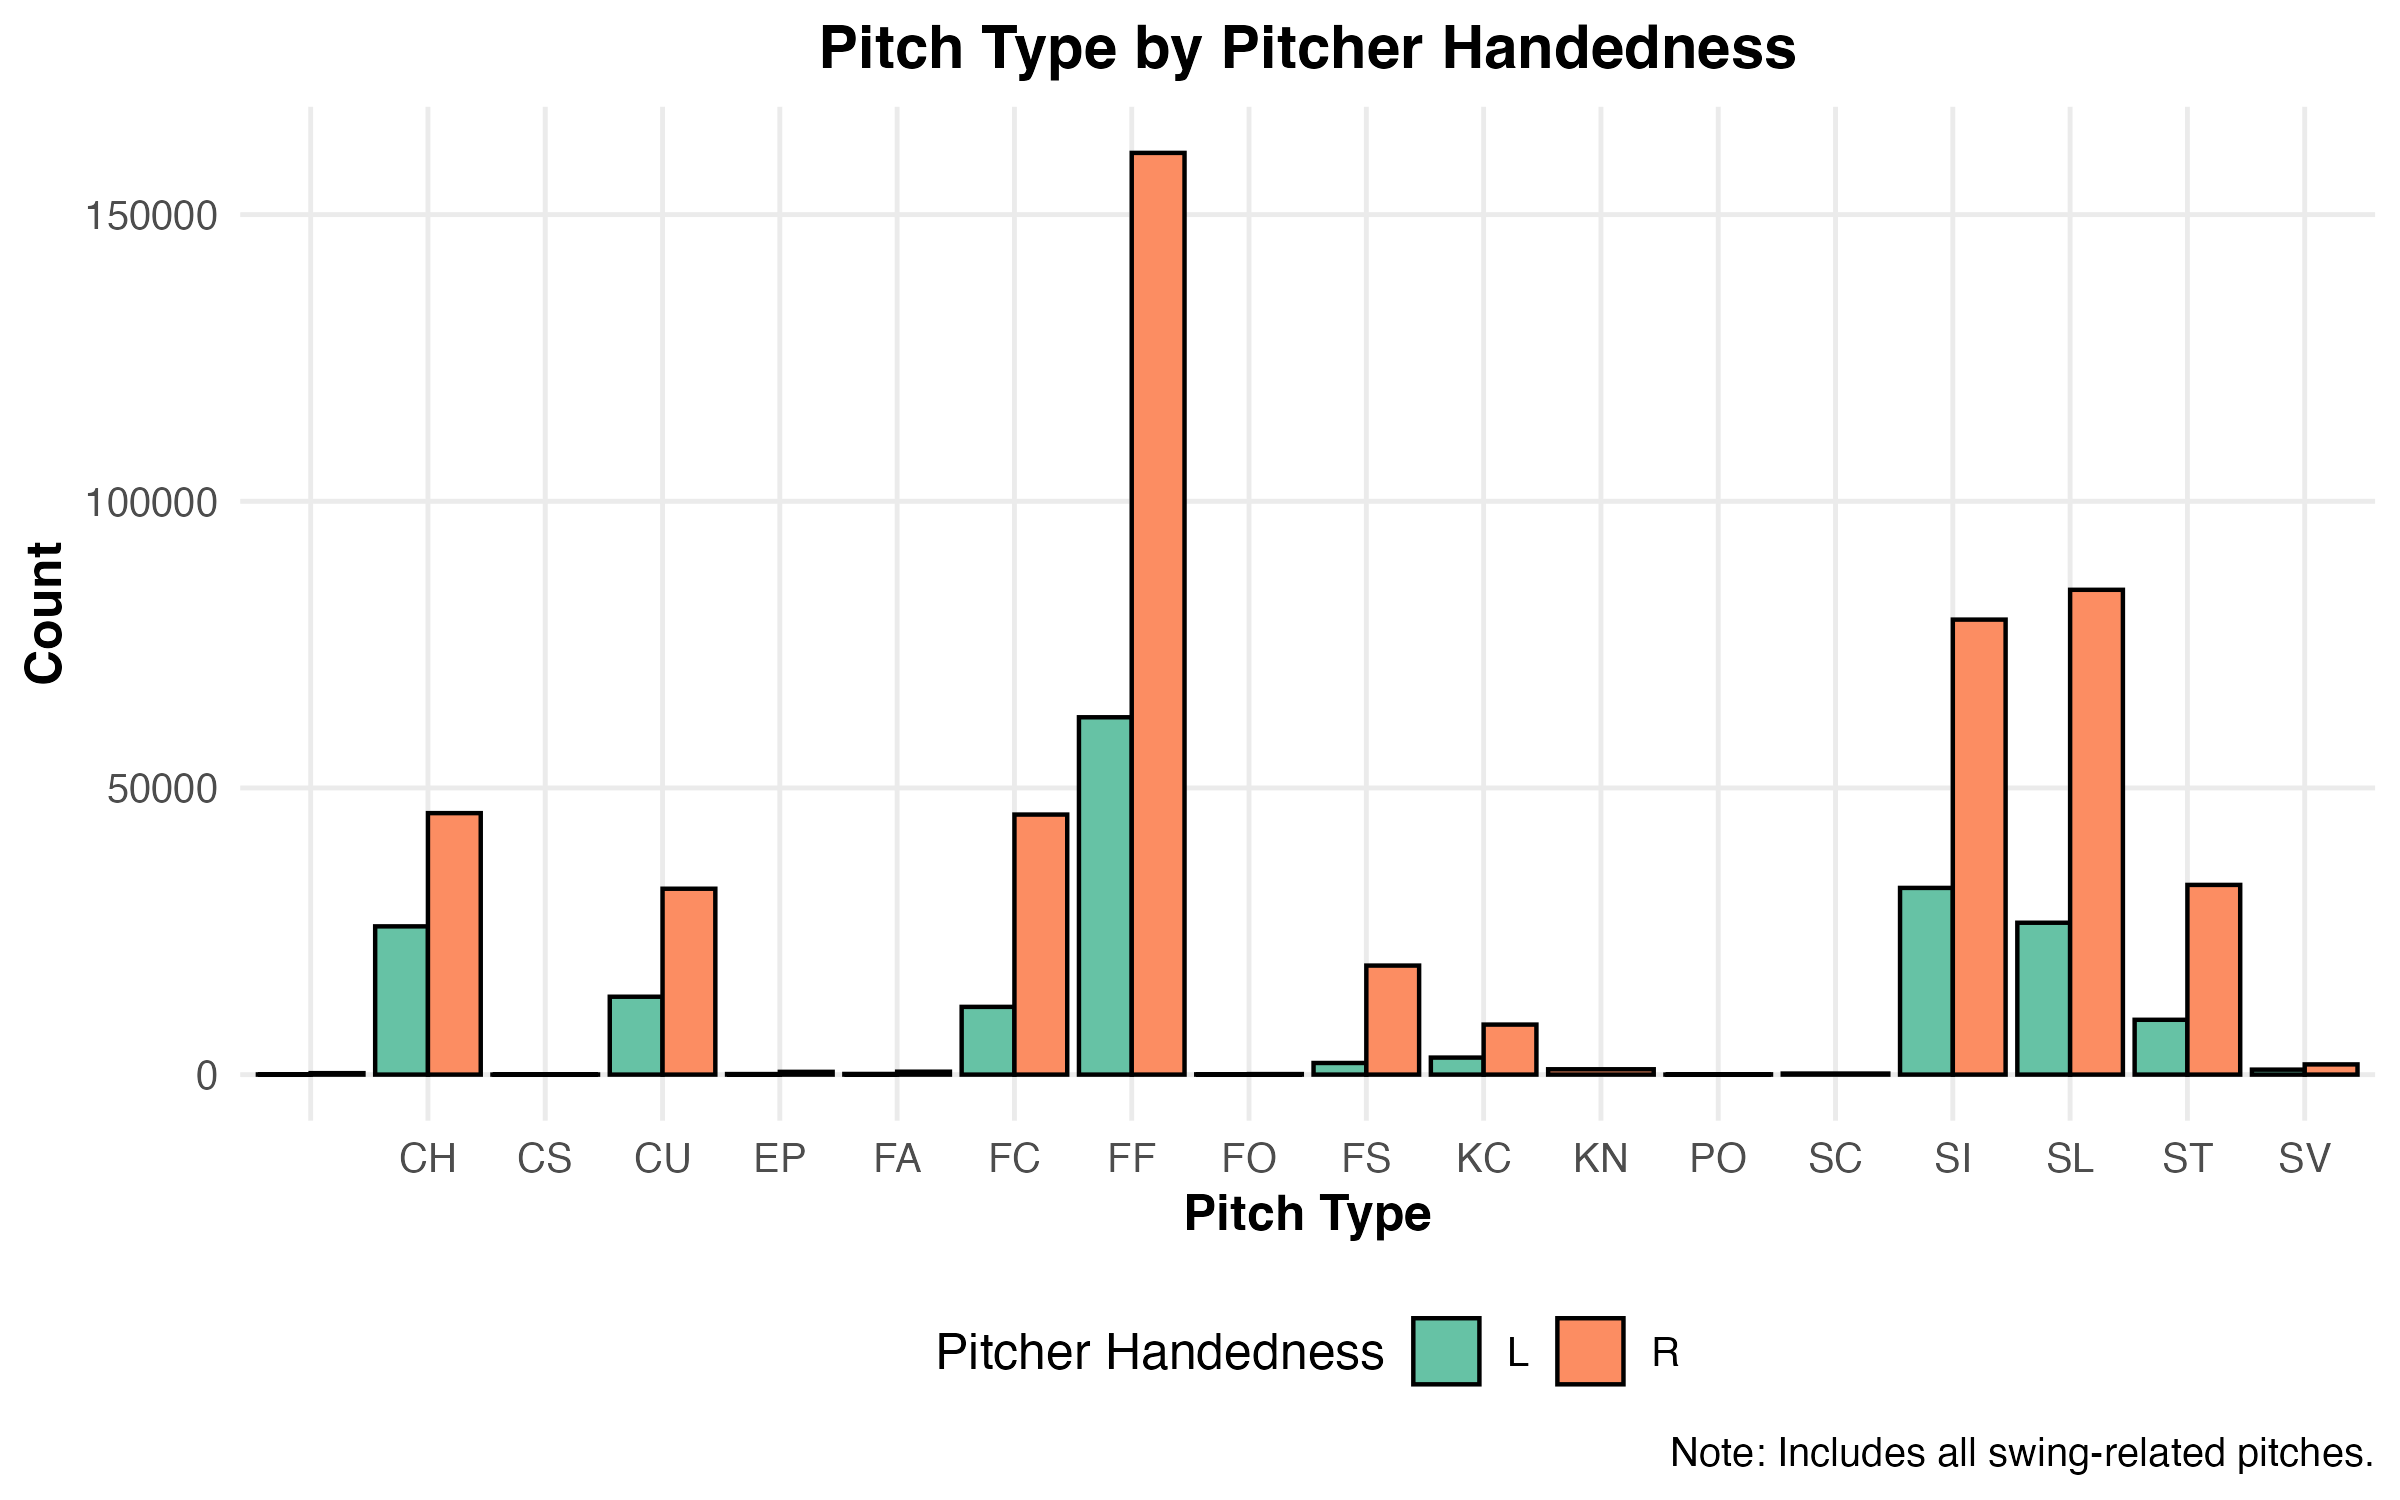
\includegraphics[width=0.8\linewidth]{pitch_hand_plot} 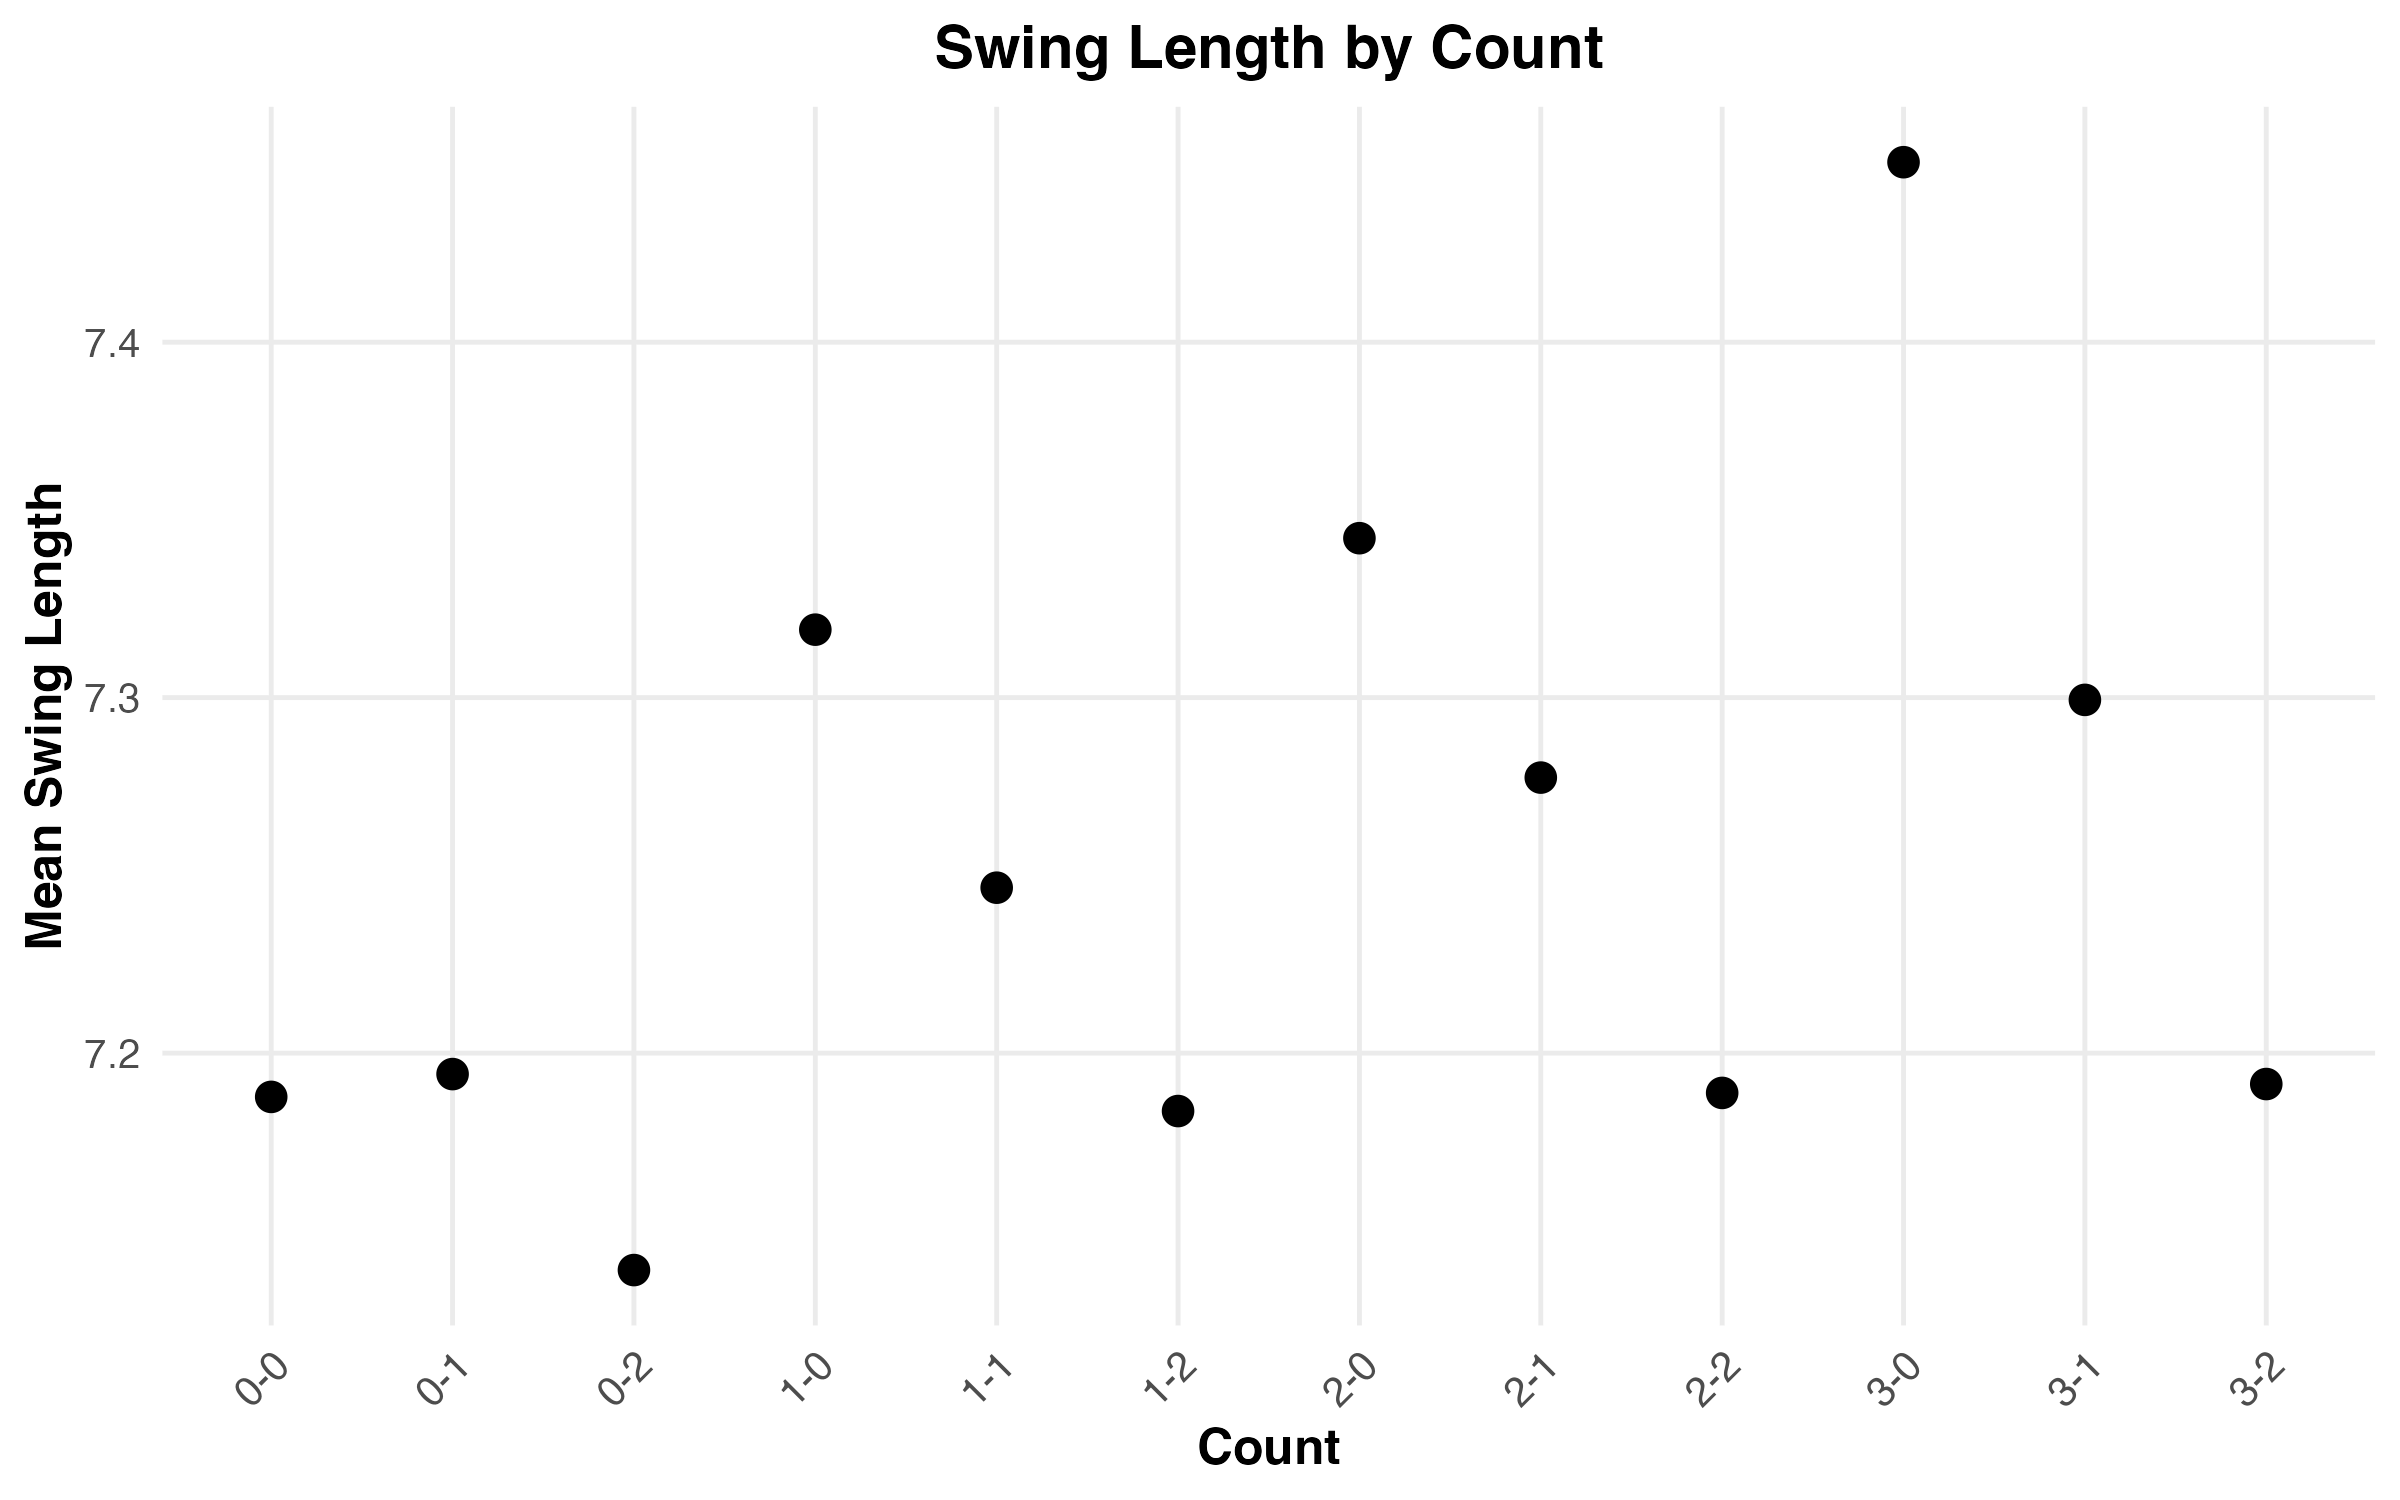
\includegraphics[width=0.8\linewidth]{swing_length_count_plot} 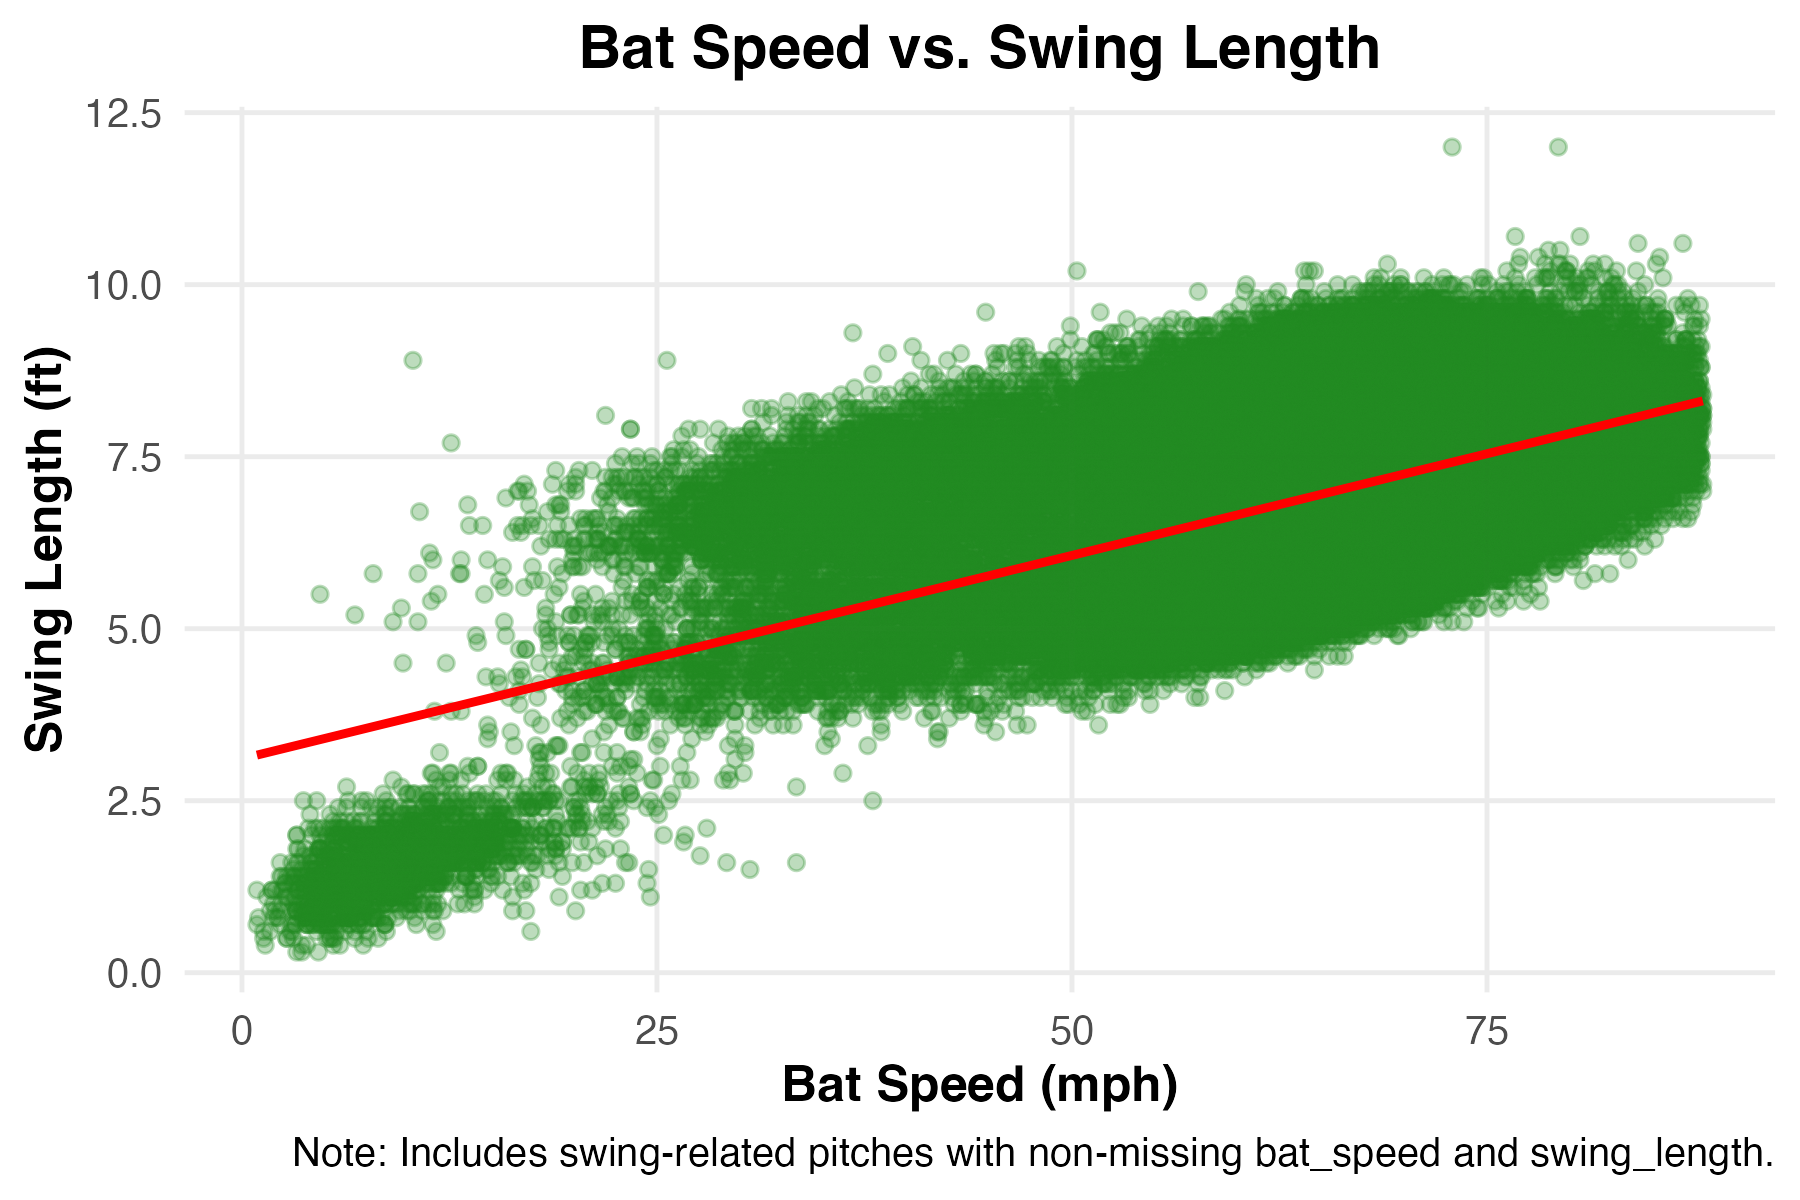
\includegraphics[width=0.8\linewidth]{swing_length_plot} \end{center}

\end{document}
